%\appendix
\chapter{Appendix A}\label{app}
	The appendix contains further details about the implementation.
	The first section adds information about the architecture of the software, the second one defines the format of the messages exchanged between client and server and the third one lists all the tools used during the development.	
			

	\section{Details About The Architecture} \label{appA}
		This section describes aspects about the design of the architecture which have been omitted in chapter \ref{chDesign}.
		In particular, it deepens the architecture of the Visual Module.
		At first it gives an overview of all the classes that compose such module and, then, it focuses on the aspects not described in the design chapter: the architecture of the Server Module and of the Utility Part of Visual Module.
		
		
		Again the description is helped by class diagrams. 
		This time, such diagrams are obtained from the source code thanks to a tool of reverse engineering.
	
		\subsection{Overview}\label{impl_arch}
		Figure \ref{fig:implementation_names} shows the class diagram of the Vision Module. 
		According to the design specifications defined in chapter \ref{chDesign}, the module is composed by the sub-modules \emph{Server} and \emph{Visual Operation}. 
		The latter is split in three parts, each one with its own tasks.

		\begin{figure}[h]
		  \begin{center} 
		    \fbox{	
		       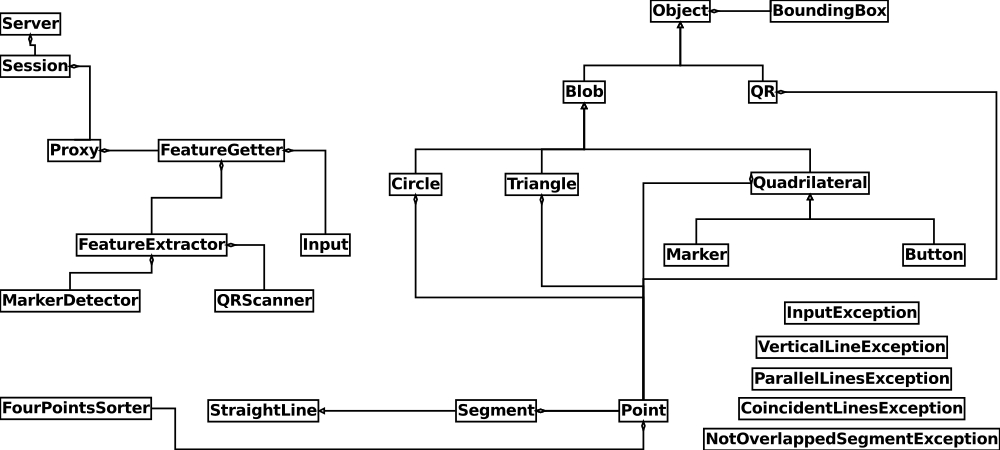
\includegraphics[width=\textwidth*\real{0.8}]{images/ch_06/implementazione_solo_nomi.jpg}
		    }
		  \end{center} 
		  \caption{\textit{Class diagram which illustrates the whole architecture of the Vision Module}}  
		  \label{fig:implementation_names}
	 	\end{figure}
 
		Classes \emph{Server} and \emph{Session} represent the Server sub-module.
		All the other classes compose the Visual Operation one.


		Classes \emph{Proxy}, \emph{FeatureGetter}, \emph{Input}, \emph{FeatureExtractor}, \emph{MarkerDetector} and \emph{QRScanner} have the role of extracting features from the input data and preparing the messages to be sent to the cognitive architecture.
		\emph{Object}, \emph{BoundingBox}, \emph{Blob}, \emph{QR}, \emph{Circle}, \emph{Triangle}, \emph{Quadrilateral}, \emph{Marker} and \emph{Button} form the object hierarchy.
		\emph{InputException}, \emph{NotOverlappedSegmentException}, \emph{ParallelLinesException}, \emph{VerticalLineException}, \emph{CoincidentLinesException}, \emph{FourPointsSorter}, \emph{StraightLine}, \emph{Segment} and \emph{Point} represent the utility classes.
	
		
		\subsection{Server Module}
		The sub-module Server, responsible for the communication with the \mbox{Lisp} interpreter, is composed by the classes \emph{Server} and \emph{Session}. 
		Figure \ref{fig:impl_feat_extraction} contains the classes that implement this service.

		\begin{figure}[h]
		  \begin{center} 
		    \fbox{	
		       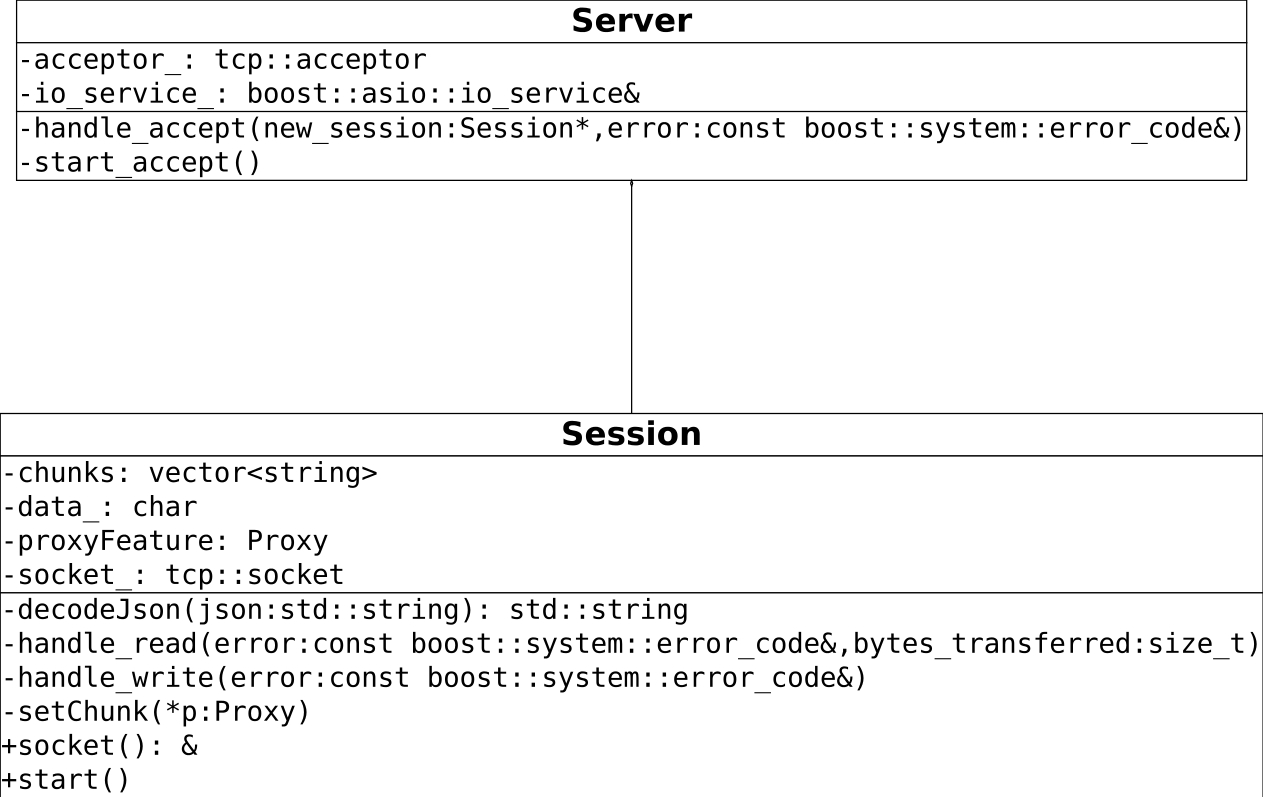
\includegraphics[width=\textwidth*\real{0.75}]{images/ch_06/communication.jpg}
		    }
		  \end{center} 
		  \caption{\textit{Class diagram describing the implementation part of the software dedicated to the communication}}  
		  \label{fig:impl_feat_extraction}
	 	\end{figure}	

		An instance of the class Server is running in background and listening for new tcp connections. 
		When a client asks for a connection, the \emph{boost::asio::io service} calls the Server callback, which creates a new instance of Session.
		The Boost library is responsible for managing either Server and Session.
		The two classes have been developed following the Boost library specifications.
		When the Session object receives a message requesting the extraction of the features, it creates an instance of Proxy and calls the proper methods of this object in order to complete its task.

		%\newpage

		\subsection{Utility Part}
		The classes which form the utility parts of the software are divided in two categories: the exception classes and the ones representing all the other utilities. 
		To these, two modules containing functions are added. 
		Figure \ref{fig:impl_utility} shows a class diagram containing all the classes that constitute this part of the software. 
		The modules, as not classes, can not be shown in the diagram but the prototypes of the functions they contain are listed below.
		
		%\subsubsection{Functions prototypes in extractorUtils.h and utils.h}
			\lstset{
				frame=single, 
				breaklines=true, 
				basicstyle=\scriptsize,
				language=c++, 
				linewidth = \linewidth,
				xleftmargin = -35pt,
				framexleftmargin= -35pt, 
				%columns=fullflexible,  
				%keepspaces=true,
				stepnumber=2, 
				%xleftmargin=-0.5in,
				%breaklines = false,
				breakautoindent = false,	
				caption=\textit{Prototypes of the functions included in extractorUtils.h and utils.h},
				morekeywords={Point,vector,cv,std},
				label=lst:proto
			}
			\begin{lstlisting}
			cv::vector<cv::vector<cv::Point> > deleteOverlapped(cv::vector<cv::vector<cv::Point> > oldList);
			cv::vector<cv::vector<cv::Point> > squaresSort(cv::vector<cv::vector<cv::Point> > squareList);
			cv::vector<cv::vector<cv::Point> > deleteFalseSquares(cv::vector<cv::vector<cv::Point> > oldList);
			cv::vector<cv::Point> sort4PointsClockwise(cv::vector<cv::Point> points);
			cv::vector<cv::vector<cv::Point> > deleteFalseTriangles(cv::vector<cv::vector<cv::Point> > oldList);
			double angle( cv::Point pt1, cv::Point pt2, cv::Point pt0 );
			double getDistance(cv::Point a, cv::Point b);
			bool similar(cv::vector<cv::Point> a, cv::vector<cv::Point> b);
			bool tooClose(cv::Point a, cv::Point b);
			bool isFalse(cv::vector<cv::Point> square);
			bool isTriangle(cv::vector<cv::Point> terna);	
			
			int getMinMax(const std::vector<Point>& coords, int type);
			std::vector<Point> sort4PointsClockwise(std::vector<Point> points);
			double erone(Point a, Point b, Point c);
			bool inLinePoints(int ax, int ay, int bx, int by, int cx, int cy );
			double getDistance(Point a, Point b);
			bool areSame(double a, double b);
			double getMin(const std::vector<double>& values);
			bool fileExists(char * path);
			string intToString(int a);\end{lstlisting}
		
		Classes \emph{InputException}, \emph{NotOverlappedSegmentException}, \emph{ParallelLinesException}, \emph{VerticalLineException} and \emph{CoincidentLinesException} are the exceptions classes. 
		As such, they are used to handle all the anomalous or exceptional events occurring at run-time.	
	
		\emph{StraightLine}, \emph{Segment} and \emph{Point} represent geometrical entities. These elements serve as basic structures for creating the objects in the hierarchy and making evaluations between couples of objects.
		Such evaluations can be both qualitative and quantitative, as, for example, the distances between the centers of two objects or the relative positions of one object in respect with another.
		
		\emph{FourPointsSorter} and the function modules contain the basic methods which are fundamental for all the operations executed by all the other classes of the software.
		For reasons of completeness the prototypes of the functions are listed in listing \ref{lst:proto}.
	

		
			
		
		\begin{figure}[h]
		  \begin{center} 
		    	
		       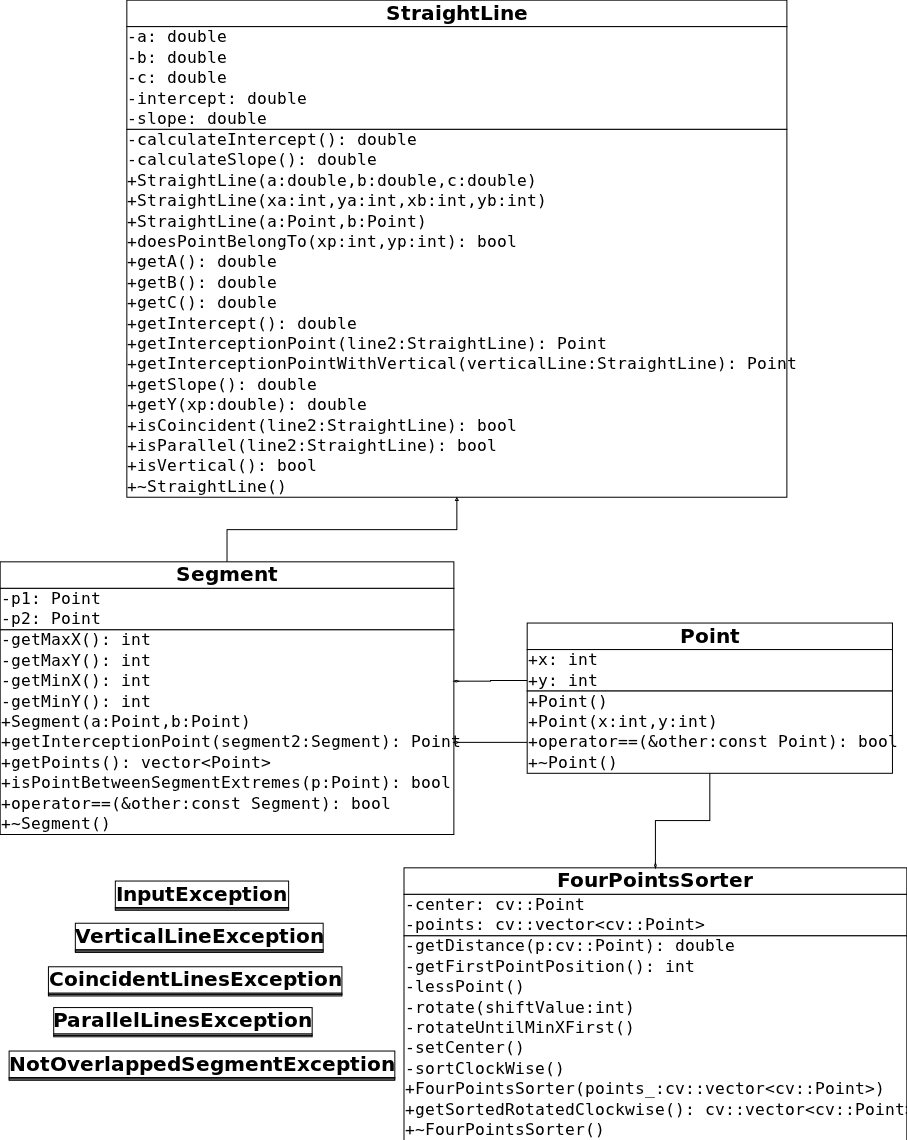
\includegraphics[width=\textwidth*\real{0.81}]{images/appendix/utility.png}
		    
		  \end{center} 
		  \caption{\textit{Class diagram showing the utility part of the Vision Module}}  
		  \label{fig:impl_utility}
	 	\end{figure}	
